\documentclass[11pt,a4paper,twoside,openright]{report}

\usepackage[top=25mm,bottom=25mm,right=25mm,left=30mm,head=12.5mm,foot=12.5mm]{geometry}
\let\openright=\cleardoublepage

\usepackage[a-2u]{pdfx}

\usepackage[
   backend=biber
%  ,style=iso-authoryear
  ,style=numeric%alphabetic
  ,citestyle=numeric
  ,sortlocale=en_US
  ,bibencoding=UTF8
  %,block=ragged
]{biblatex}
\addbibresource{references.bib}

%% Přepneme na českou sazbu, fonty Latin Modern a kódování češtiny
\usepackage[english]{babel}
\usepackage{lmodern}
\usepackage[T1]{fontenc}
\usepackage{textcomp}
\usepackage[utf8]{inputenc}

% Set fonts
%\RequirePackage[osf]{mathpazo} % Palatino with oldstyle figures
%\newcommand\liningnums[1]{\fontfamily{ppl}\selectfont#1}
%\RequirePackage{eulervm}
%\RequirePackage[scaled=.8819]{sourcecodepro} % Source Code Pro typeface for monospace

%%% Další užitečné balíčky (jsou součástí běžných distribucí LaTeXu)
\usepackage{amsmath}        % rozšíření pro sazbu matematiky
\usepackage{amsfonts}       % matematické fonty
\usepackage{amsthm}         % sazba vět, definic apod.
\usepackage{bm}             % tučné symboly (příkaz \bm)
\usepackage{graphicx}       % vkládání obrázků
\usepackage{fancyvrb}       % vylepšené prostředí pro strojové písmo
\usepackage{fancyhdr}       % prostředí pohodlnější nastavení hlavy a paty stránek
\usepackage{icomma}         % inteligetní čárka v matematickém módu
\usepackage{dcolumn}        % lepší zarovnání sloupců v tabulkách
\usepackage{booktabs}       % lepší vodorovné linky v tabulkách
\makeatletter
\@ifpackageloaded{xcolor}{
   \@ifpackagewith{xcolor}{usenames}{}{\PassOptionsToPackage{usenames}{xcolor}}
  }{\usepackage[usenames]{xcolor}} % barevná sazba
\makeatother
\usepackage{multicol}       % práce s více sloupci na stránce
\usepackage{caption}
\usepackage{enumitem}
\usepackage{lipsum}
\setlist[itemize]{noitemsep, topsep=0pt, partopsep=0pt}
\setlist[enumerate]{noitemsep, topsep=0pt, partopsep=0pt}
\setlist[description]{noitemsep, topsep=0pt, partopsep=0pt}
\usepackage{pdfpages}

\usepackage{tocloft}
\setlength\cftparskip{0pt}
\setlength\cftbeforechapskip{1.5ex}
\setlength\cftfigindent{0pt}
\setlength\cfttabindent{0pt}
\setlength\cftbeforeloftitleskip{0pt}
\setlength\cftbeforelottitleskip{0pt}
\setlength\cftbeforetoctitleskip{0pt}
\renewcommand{\cftlottitlefont}{\Huge\bfseries}
\renewcommand{\cftloftitlefont}{\Huge\bfseries}
\renewcommand{\cfttoctitlefont}{\Huge\bfseries}

% vyznaceni odstavcu
\parindent=0pt
\parskip=11pt

% zakaz vdov a sirotku - jednoradkovych pocatku ci koncu odstavcu na prechodu mezi strankami
\clubpenalty=1000
\widowpenalty=1000
\displaywidowpenalty=1000

% nastaveni radkovani
\renewcommand{\baselinestretch}{1.20}

% nastavení hlavy a paty stránek
\fancyhf{}
\renewcommand{\chaptermark}[1]{\markboth{#1}{}}
\fancyhead[RO,LE]{\leftmark}
\fancyfoot[RO,LE]{\thepage}
%\renewcommand{\footrulewidth}{0pt}
\fancypagestyle{plain}{%
\fancyhf{} % clear all header and footer fields
\fancyfoot[RO,LE]{\thepage}
\renewcommand{\headrulewidth}{0pt}
%\renewcommand{\footrulewidth}{0.5pt}
}

% Tato makra přesvědčují mírně ošklivým trikem LaTeX, aby hlavičky kapitol
% sázel příčetněji a nevynechával nad nimi spoustu místa. Směle ignorujte.
\makeatletter
\def\@makechapterhead#1{
  {\parindent \z@ \raggedright 
   \Huge\bfseries \thechapter. #1
   \par\nobreak
   \vskip 20\p@
}}
\def\@makeschapterhead#1{
  {\parindent \z@ \raggedright 
   \Huge\bfseries #1
   \par\nobreak
   \vskip 20\p@
}}
\makeatother

% Trochu volnější nastavení dělení slov, než je default.
\lefthyphenmin=2
\righthyphenmin=2

% Zapne černé "slimáky" na koncích řádků, které přetekly, abychom si
% jich lépe všimli.
\overfullrule=1mm

%% Balíček hyperref, kterým jdou vyrábět klikací odkazy v PDF,
%% ale hlavně ho používáme k uložení metadat do PDF (včetně obsahu).
%% Většinu nastavítek přednastaví balíček pdfx.
\hypersetup{unicode}
\hypersetup{breaklinks=true}
\hypersetup{hidelinks}

%%% Prostředí pro sazbu kódu, případně vstupu/výstupu počítačových
%%% programů. (Vyžaduje balíček fancyvrb -- fancy verbatim.)

\DefineVerbatimEnvironment{code}{Verbatim}{fontsize=\small, frame=single}

% \coloneqq and other symbols
\usepackage{mathtools}

% name of the project
\newcommand\pname{brandy0}

\newcommand\this{project}
\newcommand\software{software}
\newcommand\vxlisp{\vspace*{12pt}}
\newcommand\icd[1]{\texttt{#1}}
\newcommand{\ccd}[1]{\colorbox{gray!15!white}{\texttt{#1}}}
\newcommand{\scd}[1]{
	\vspace*{5pt}

	\ccd{#1}
	\vspace*{5pt}
}
\newcommand{\nscd}[1]{\scd{\$ #1}}
\newcommand{\sscd}[1]{\scd{\$ sudo #1}}
\newcommand{\aptinstall}[1]{\sscd{apt install #1}}
\newcommand{\snapinstall}[1]{\sscd{snap install #1}}
\newcommand{\defos}{Ubuntu 20.10}
\newcommand{\psubinst}{possible installation using \icd{snap} on \defos}
\newcommand{\pubinst}{possible installation using \icd{apt} on \defos}

\newcommand\dt{\Delta t}
\newcommand\dx{\Delta x}
\newcommand\dy{\Delta y}

%\newcommand\vxpder[2]{\frac{\partial #1}{\partial #2}}


\def\NazevPrace{Název maturitní práce}
\def\Trida{R8.A}
\def\AutorPrace{Viktor Fukala}
\def\DatumOdevzdani{2021}

% Vedoucí práce: Jméno a příjmení s~tituly
\def\Vedouci{Šimon Schierreich} % TODO dodat tituly

% Studijní program a obor
\def\StudijniProgram{studijní program}
\def\StudijniObor{studijní obor}

% Text čestného prohlášení
\def\Prohlaseni{Prohlašuji, že jsem svou práci vypracoval samostatně a použil jsem pouze prameny a literaturu
uvedené v~seznamu bibliografických záznamů. Nemám žádné námitky proti zpřístupňování této práce v~souladu se
zákonem č. 121/2000 Sb. o~právu autorském, o~právech souvisejících s~právem autorským a
o~změně některých zákonů (autorský zákon) ve znění pozdějších předpisů.}

% Text poděkování
\def\Podekovani{%
Poděkování.
}

% Abstrakt česky
\def\Abstrakt{%
Abstrakt.
}

% Abstrakt anglicky
\def\AbstraktEN{%
The \software{} developed in this \this{}, \pname{}, is a native application for Linux and Windows that predicts and visualizes the flow of an incompressible fluid around arbitrary obstacles and under various conditions in two-dimensional space. It aims to deepen the basic understanding of fluid flow among its end-users by presenting physically accurate visualizations without the sophisticated interface that often comes with fluid simulation software used in the industry. It simulates the flow based on the shapes of the obstacles and the boundary conditions for pressure and velocity, all of which can be configured by the end-user before starting the simulation. The \software{} works the fastest and most reliably for low Reynold numbers (laminar flow), whereas for high Reynold numbers (turbulent flow), the amount of required computational resources (both in time and space) increases rapidly. Nevertheless, the \software{} achieves its goal by being able to simulate a wide range of laminar flows and phenomena (such as the development of vortices) during at the transition to turbulent flows.
}

% 3 až 5 klíčových slov
\def\KlicovaSlova{klíčové slovo, další pojem, jiný důležitý termín, a ještě jeden}
% 3 až 5 klíčových slov anglicky
\def\KlicovaSlovaEN{computational fluid dynamics, incompressible Navier-Stokes equations, visualization, computer simulation}


\begin{document}

%%% Titulní strana práce a další povinné informační strany

%%% Titulní strana práce

\pagestyle{empty}
\pagenumbering{gobble}
\hypersetup{pageanchor=false}

\begin{center}
\LARGE
\textbf{GYMNASIUM JANA KEPLERA}\\
{\large Parléřova 2/118, 169 00 Praha 6}

\vspace{\stretch{3}}

\includegraphics[width=.3\textwidth]{img/logo}

\vspace{\stretch{3}}

{\Huge\bfseries\NazevPrace}

\vspace{8mm}
\mdseries{Maturita Project}

\vspace{\stretch{8}}
\large
\begin{tabular}{rl}
Author: & \AutorPrace \\
\noalign{\vspace{2mm}}
Class: & \Trida\\
\noalign{\vspace{2mm}}
School year: & 2020/2021\\
\noalign{\vspace{2mm}}
Subject: & Computer Science \\
\noalign{\vspace{2mm}}
Supervisor: & \Vedouci \\
\end{tabular}

\vspace{20mm}
Prague, \DatumOdevzdani
\end{center}


\openright

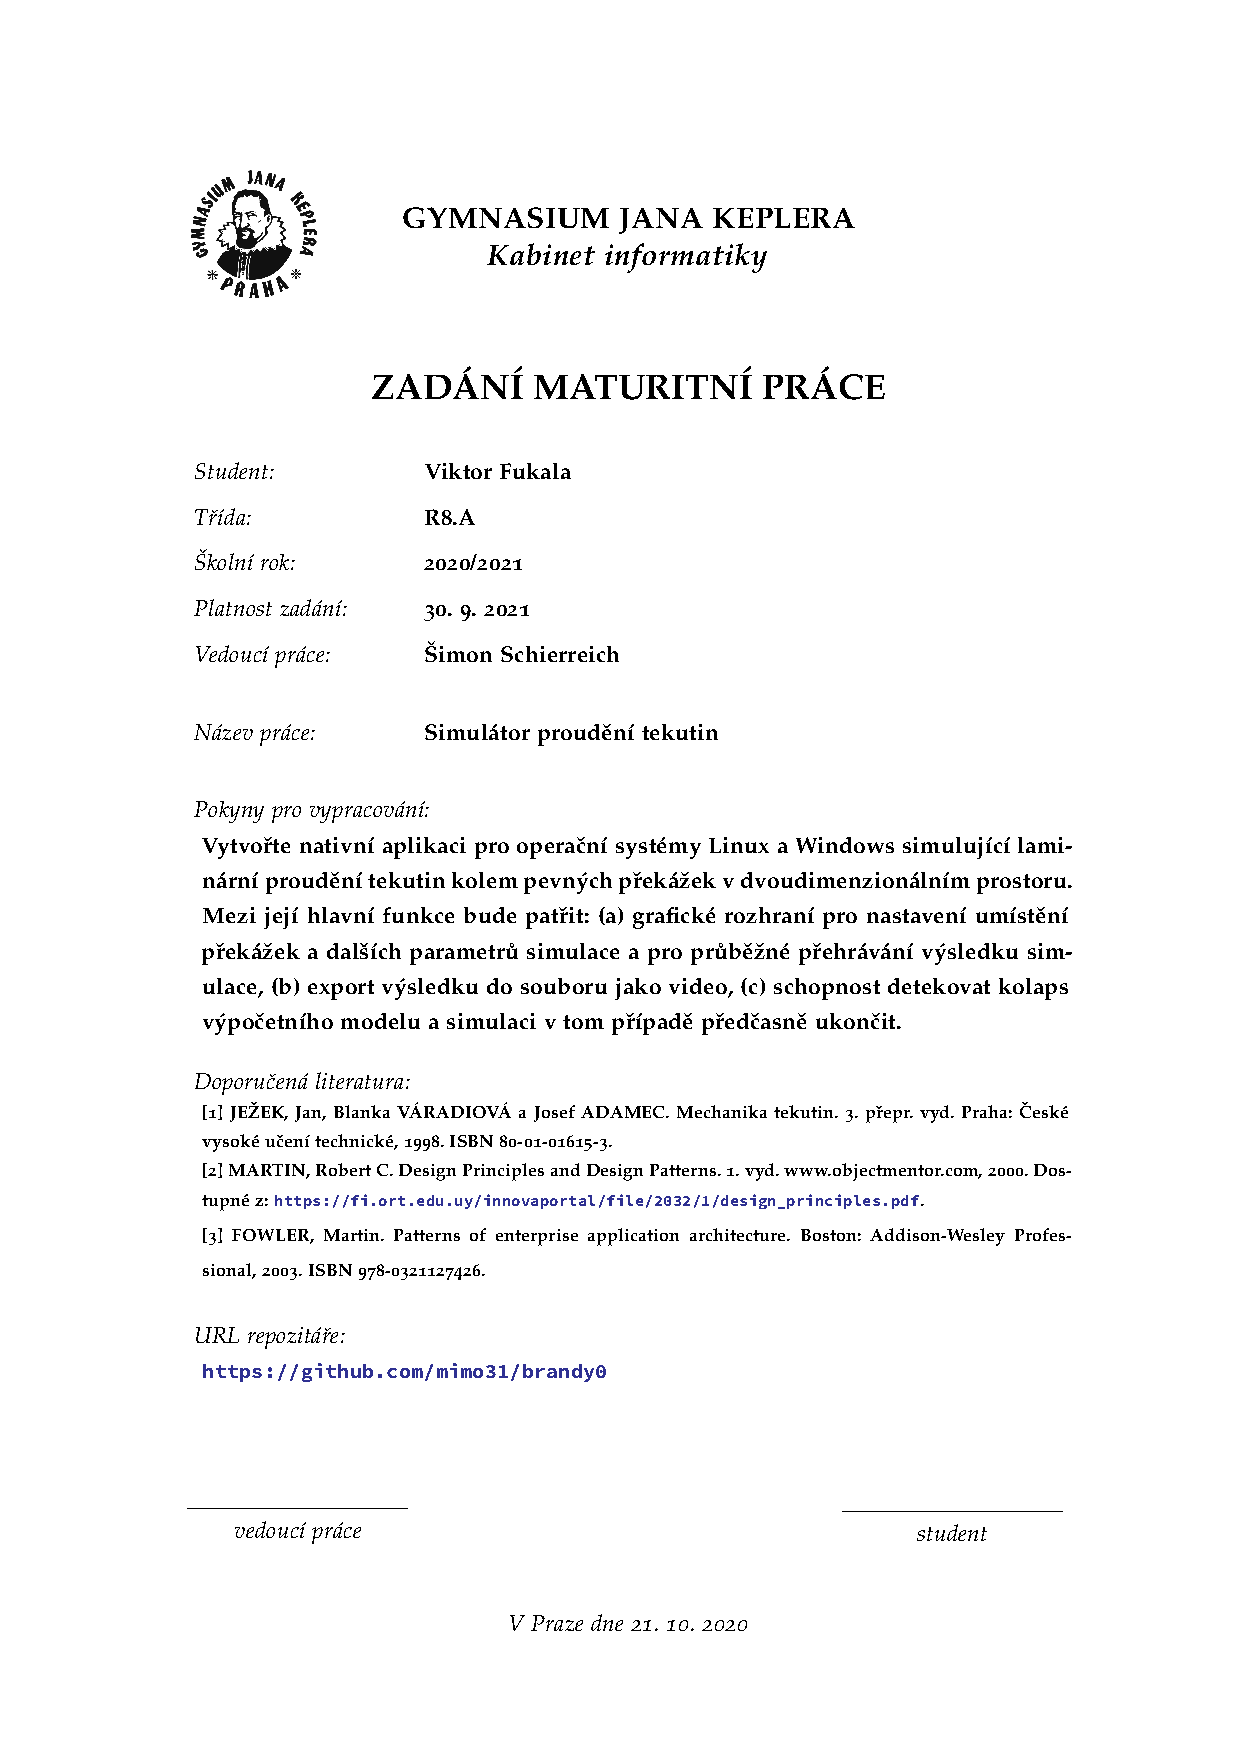
\includepdf[]{zadani.pdf}


%%% Strana s čestným prohlášením k bakalářské práci

\hypersetup{pageanchor=true}
\cleardoublepage
\vspace*{\fill}
\section*{Declaration of Authorship}
\noindent
\Prohlaseni

\vspace{2cm}
\noindent
Prague, \today
\hspace*{\fill}\small{\AutorPrace}
\vspace{1cm}

%%% Poděkování
\openright
\vspace*{\fill}
\section*{Acknowledgements}
\noindent
\Podekovani
\vspace{1cm}


%%% Povinná informační strana bakalářské práce
\openright
\section*{Abstrakt}
\noindent
\Abstrakt
\subsection*{Klíčová slova}
\noindent
\KlicovaSlova

\bigskip\bigskip\bigskip
\section*{Abstract}
\noindent
\AbstraktEN
\subsection*{Keywords}
\noindent
\KlicovaSlovaEN

\openright
\pagenumbering{arabic}


% Obsah
\setcounter{tocdepth}{2}
\tableofcontents

\newcommand{\dt}{\Delta t}

\chapter{Theoretical Background}
\pagestyle{fancy}

\section{Introduction}
Computational fluid dynamics (CFD) is the application of numerical methods to fluid flow problems. As of today, it plays a vital role in engineering areas and the related industries such as aeronautics, the automotive industry, environmental engineering, bioengineering (simulating the blood flow or the air flow in lungs, for example), or even videogames, where it is used to produce realistic video of fluids. Computer-simulated fluid flow has replaced many expensive or even technically infeasible real-world experiments, and its importance is only expected to grow with future advancements in both computing power and the efficiency of the applied algorithms.

In this \this{} however, we are not focused on any of these direct applications but rather on providing the end-user with the fundamental understanding of fluid flow phenomena and a high degree of freedom in experimenting -- i.e.\ setting up simulations to their liking. We aim to present \software{} that visualizes the computed results in an attractive and immediate manner, so that our goals differ greatly from those of the software used in the industry, as that often prioritizes precision and efficiency and comes with an elaborate user interface and special functionality for the one or the other engineering or industry application.

My main motivation for committing myself to the development of the \software{} constituting this \this{} was my fascination with the computers' ability to simulate (parts of) the real world and my curiosity as to how far one can get with only the general knowledge of physics and numerical analysis fundamentals and no prior expertise in CFD specifically.

Our \software{} computes and visualizes the temporal evolution of the state of a fluid inside a two-dimensional, rectangular container. The state of the fluid is given by the velocity vector field and the pressure scalar field, each of which has a value at every point inside the container. This state at some given time after the start of the simulation is dependent on a multitude of parameters:
\begin{itemize}
	\item \textbf{the shape of the container,}\\
		This includes the dimensions of the rectangular enclosing container and also the shapes and dimensions of the solid obstacles inside it. Both can be freely configured by the end-user before a simulation.
	\item \textbf{the mechanical properties of the fluid,}\\
		This includes the density and the viscosity of the fluid, of which both can be freely configured by the end-user.
	\item \textbf{the boundary conditions at the boundary of the container, and}\\
		At the four sides of the outer container, the user can specify what boundary conditions will be enforced. For both velocity and pressure, they can choose between a Dirichlet type or a Neumann type boundary condition. For the Dirichlet type boundary condition, they can also specify the value (of pressure or velocity) at the boundary. Under a Neumann type boundary condition we specifically understand a the Neumann boundary conditions which requires the derivative along the normal to the surface to be zero.
		\vxlisp

		At the inner boundaries, i.e.\ at the surface of the solid obstacles inside the container, the no-slip condition is enforced for velocity (meaning that a Dirichlet type boundary condition setting the velocity to the zero vector holds) and a Neumann type boundary conditions is set for pressure.
	\item \textbf{the initial conditions.}\\
		I.e.\ the state of the fluid at $t=0$. The state of the fluid at $t=0$ is set to zero velocity and zero pressure everywhere (except at the boundary).
\end{itemize}

\section{Physical Model}
To model the behavior of the fluid, we use the Navier-Stokes equations. Let $\mathbf u$ denote the velocity of the fluid and $p$ its pressure at all the points inside the container. We assume that the fluid is incompressible, so we get the incompressibility equation
\newcommand{\uu}{\mathbf u}
\newcommand{\D}{\mathrm D}
\begin{align}\label{eq:incom}
	\nabla\cdot\uu=0.
\end{align}
Then we have the Navier-Stokes momentum equation
\newcommand{\conv}{\frac{\D\uu}{\D t}}
\begin{align*}
	\rho\conv=-\nabla p+\mu\nabla^2\uu+\rho\mathbf g,
\end{align*}
where $\rho$ is the density of the fluid, $\mu$ its (dynamic) viscosity, $\mathbf g$ is the acceleration due to external forces (such as gravity) and $\conv$ denotes the material (also known as \emph{convective}) derivative of the velocity.
\newcommand{\pder}[2]{\frac{\partial #1}{\partial #2}}
\begin{align}
	\conv=\pder\uu t+(\uu\cdot\nabla)\uu
\end{align}
We assume no external forces, so $\mathbf g=0$. Hence, the momentum equation that we work with takes the form
\begin{align}\label{eq:momentum}
	\pder\uu t+(\uu\cdot\nabla)\uu=-\frac1\rho\nabla p+\nu\nabla^2\uu,
\end{align}
where $\nu=\mu/\rho$ is the \emph{kinematic} viscosity.
\section{Numerical Model}
% TODO: add citation
[add citation to Barba's materials; mention what her and this model have in common and how they differ]
Our way of numerically solving the above equations that is not the most accurate or computationaly efficient, but it is relatively simple to implement and to work with. It can be categorized as an explicit finite difference method.

Let us denote the value of a particular quantity at the $i$-th iteration by $i$ in the superscript. That is, let $\uu^i$ be the velocity field at the $i$-th iteration, $p^i$ the pressure field at the $i$-th iteration, $\left(\pder\uu t\right)^i$ the time derivative of the velocity field at the $i$-th iteration. Then we approximate the derivate of $\uu$ by the forward difference.
\begin{align}
	\left(\pder{\uu}t\right)^i=\frac{\uu^{i+1}-\uu^i}{\dt}
\end{align}
So at the $i$-th iteration, \eqref{eq:momentum} takes the form
\begin{align}
	\frac{\uu^{i+1}-\uu^i}{\dt}+(\uu^i\cdot\nabla)\uu^i=-\frac1\rho\nabla p^i+\nu\nabla^2\uu^i.
\end{align}
Together with the equation $\nabla\cdot\uu^{i+1}=0$ (that is \eqref{eq:incom} at the $(i+1)$-th iteration), this allows us to solve for $\uu^{i+1}$ and $p^i$. We express
\begin{align}
	\uu^{i+1}=-\frac\dt\rho\nabla p^i+\dt\left(\nu\nabla^2\uu^i-(\uu^i\cdot\nabla)\uu^i\right)+\uu^i.
\end{align}
During the computation, we have yet to solve for $p^i$, so we only calculate the following intermediate vector field
\newcommand{\ww}{\mathbf w}
\begin{align*}
	\ww^i\coloneqq\dt\left(\nu\nabla^2\uu^i-(\uu^i\cdot\nabla)\uu^i\right)+\uu^i
\end{align*}
The above formula gives the value of the field in the interior of the grid and we use the boundary conditions for velocity to calculate its values at the boundary. Then
\begin{align*}
	-\frac\dt\rho\nabla p^i+\ww^i=\uu^{i+1}
\end{align*}
and
\begin{align*}
	-\frac\dt\rho\nabla^2p^i+\nabla\cdot\ww^i=\nabla\cdot\uu^{i+1}=0.
\end{align*}
Hence, we have the following Poisson equation for $p^i$
\begin{align*}
	\nabla^2p^i=\frac\rho\dt\nabla\cdot\ww^i.
\end{align*}
We solve this Poisson equation\footnote{There exist several well-known methods for solving a Poisson equation numerically. They include, most notably, the Jacobi method, the Gauss-Seidel method, successive over-relaxation, and multigrid methods. Multigrid methods generally coverge the fastest, but are noticeably more complex and difficult to implement than the other approches mentioned. Of those, we use successive over-relaxation by default as it tends to have the fastest convergence.} for $p^i$ in the interior of our grid and apply the boundary conditions for pressure to obtain $p^i$ at the boundary.
%\vxlisp

At last, we compute $\uu^{i+1}$ given by
\begin{align*}
	\uu^{i+1}=-\frac\dt\rho\nabla p^i+\ww^i
\end{align*}
and the boundary conditions for velocity.

V první části maturitní práce by se měla objevit informace o tom, jaký problém řešíte. Co si Váš projekt klade za cíl?

\chapter{Implementation}

\section{Used Technologies}
\subsection{Base Programming Language: C++}
The \software{} is written mostly in C++. C++ is a compiled programming language with multiple freely available compilers, which are capable of many optimizations, so that the resulting executable programs are one of the fastest when compared to other programming languages. This is important for us because computational resources (and their efficient use) are a limiting factor during the simulations. Moreover, C++ code can be written in a highly structured manner (e.g.\ using objects and classes, namespaces, templates, \icd{constexpr}, \icd{const}, static assertions, etc.), which decreases the likelihood of errors altogether or at least enables better static analysis and the discovery of potential errors at compile time (compared to the C programming language, for example). 

\subsection{User Interface, Widget Toolkit}
The most visible technology used in the \software{} is gtkmm 3, a C++ wrapper around GTK+ 3 user interface widget toolkit library. It is one of the two most widely used user interface libraries for C++, the other being Qt. Qt is written natively in C++ (in contrast to GTK being a C library), but the gtkmm wrapper for C++ makes good use of C++ paradigms, so that gtkmm interoperates with C++ code just as easily. Hence, both gtkmm and Qt seemed adequate for our \software{} and the final decision was based on a personal preference for the GNOME ecosystem.

\subsection{OpenGL for Visualizations}
Specifically for the visualization of the simulated fluid flow, we use OpenGL to produce detailed images accurately representing the computed states easily and to do so fast enough to be able to play the images as a continuous video. No complex graphics was necessary for our \software{}, so only 4 relatively simple shaders written in the OpenGL Shading Language are a part of the source code.

\subsection{FFmpeg for Writting Video Files}
% TODO: add link
Since the \software{} was required to be able to produce video files with the visualized flow of the fluid, we used the FFmpeg libraries for video manipulation. See [link here to installation -- ffmpeg libs] for the exact information about the FFmpeg libraries used. Even though these are C libraries and so their API violates the principles of good design in C++, we use them because they are one of the most widely used tools for this kind of tasks and we are able to keep the iteraction with their API local within our codebase.

Druhá kapitola obsahuje detailní informace o tom, jak probíhala implementace. Zde se objeví zdůvodnění výběru technologií, řešení problémů, na které jste narazili, informace o použitých knihovnách apod. Pochvalte se, nikdo to za Vás neudělá. Přiznejte chyby, není to ostuda.

\subsection{CMake for Build Management}

\section{Course of Development}
% TODO: add citations
At the beginning (September 2020 -- November 2020), we searched for and tried multiple physical models (e.g.\ incompressible or compressible fluid) and numerical models (various computation schemes) and we researched other software that already solves problems similar to what we aimed to do. There certainly exist other similar programs such as Flowsquare [add citation] or OpenFOAM [add citation]. Both of these are generaly allow for more sophisticated simulations, but they also typically require configuration outside of the program's own interface (e.g.\ preparation of bitmaps file with solid obstacles (Flowsquare) or writting the complete simulation setup into a configuration file (OpenFOAM)). Our software tries to be more accessible for less technically skilled users.

% TODO: add citations, add image
For the sake of simplicity, we started to focus only on incompressible flow. Besides Wikipedia articles such as [add citation for wiki pages: Navier-Stokes equation, Jacobi method, Gauss-Siedel method, Successive over-relaxation], the most useful source of practical information were Lorena A. Barba's materials on CFD [add citation to 12 steps to Navier-Stokes] and the recordings of her CFD course at Boston University [add citation to YouTube playlist]. Throughout these initial stages of the development, we needed to perform many experiments in order to determine how reliably our numerical models work. A sizeable portion of them were unstable and resulted in the computation diverging [add image of a diverging simulation]. Generally, we can say that none of our models (including the final one) could efficiently simulate turbulence (flow with a high Reynolds number).

In December, the development continued with the implementation of the main parts of the simulation configuration interface and the OpenGL visualization. The inteface for the configuration of solid obstacles was implemented mainly in January and in February, controls for the video playback and the option to export video were added. Throughout March, parts of the numerical model were improved (including its efficiecy), more options for the configuration of boundary conditions were made possible and various minor parts of the \software{} were improved, expanded, or fixed.

\section{Elegant and Efficient Solutions during Development}
This section discusses a few parts of the project that could be regarded as well tackled or as problems elegantly solved.

\subsection{Obstacle Configuration Interface}
One could argue that the obstacle configuration interface is, in contrast to other components of the \software{}, elegant and user-friendly. It displays to the user the obstacle they are about to add and the grid points that will become solid as a result of that, it allows them to sequentially undo and redo the addition of obstacle, or it allows to cancel the addition of a new obstacle. However, this might be, in part, caused by the relative isolation and clearly defined bound of this interface is supposed to do in the first place, particularly when the rest, the majority, and the core of the \software{} is rather volatile.

Nevertheless, there is room for improvement even in this interface. For example, the performance (and thus the smoothness of the UI) worsens as the number of points grows large enough and the editor lacks any ability to copy or move the added obstacles.

\subsection{Use of C++ Paradigms}
It is highly debatable claim to say that in general, the structure of the codebase is well design. But let us draw the attention to at least some specific part of the code that one may regard as well-design.

Firstly, notice the structs defined in the \icd{lib} directory -- namely \icd{Grid}, \icd{vec2d}, \icd{Point}. The \icd{Grid} struct is a generic two-dimensional container of fixed size and is used to represent the values of a quantity at the grid points inside a container. The \icd{vec2d} struct is a representation of a two-dimensional vector (with two coordinates of type \icd{double}) and \icd{Point} of a point with two integer coordinates. All these structs make heavy use of operator overloading, so that they can be used more easily and naturaly. That includes a natural way of addressing the data in a \icd{Grid}, so that statements like
\begin{align*}
	\icd{g(3, 4) = g(0, 1)}
\end{align*}
or even
\begin{align*}
	\icd{g(p1) = g(p0)},
\end{align*}
where \icd g is of type \icd{Grid<T>} for any type \icd{T} that is copy assignable and $\icd{p0}$, $\icd{p1}$ are of type $\icd{Point}$, can be used (provided that the specified indices or points are within the bounds of the grid). Naturally, standard vector operation are also available through overloaded operators, so
\begin{align*}
	&\icd{p = (u.dot(a) / u.dot(u)) * u}\\
	&\icd{d = (a + b) / 2 + c * 1.5}
\end{align*}
are valid statements for \icd a, \icd b, \icd c, \icd d, \icd p, \icd u of type \icd{vec2d}.

On a similar note, we implemented a generic class \icd{Hideable} (in \icd{hideable.hpp}), which allows us to hide a GTK widget while it still takes up space in its parent container. The elegance of this generic class is that \icd{Hideable<T>} inherits from \icd T, so that a widget of type \icd W can be declared as \icd{Hideable<W>} and all its methods and attributes are still accessible normally while it now also has the new methods that hide and show (unhide) it.

However, other parts of the codebase are not so well designed. For example, the classes representing the program's windows and the classes representing the various stages of configuring / running a simulation try to follow a general pattern, but mainly due to the large number of different states the user interface can be in, they contain a relatively high amount of loosely structured code.

\chapter{User Guide}

Poslední kapitola obsahuje informace o tom, jak projekt, který v rámci maturitní práce vznikl, nainstalovat, spustit a používat.

\section{Ukázka sekce}

\lipsum[5]

\subsection{A jedné podsekce}

\lipsum

\section{A další sekce}

\lipsum

\chapter*{Závěr}
\pagestyle{empty}
\addcontentsline{toc}{chapter}{Závěr}

Závěr obsahuje shrnutí práce a vyjadřuje se k míře splnění jejího zadání. Dále by se zde mělo objevit sebehodnocení studenta a informace o tom, co nového se naučil a jak vnímal svou práci na projektu.

%%% Seznam použité literatury
\nocite{einstein}\nocite{latexcompanion}\nocite{knuthwebsite}
\printbibliography[title={Seznam použité literatury},heading={bibintoc}]

%%% Seznam obrázků
\openright
\listoffigures
\addcontentsline{toc}{chapter}{Seznam obrázků}

%%% Seznam tabulek
\clearpage
\listoftables
\addcontentsline{toc}{chapter}{Seznam tabulek}

%%% Přílohy k práci, existují-li. Každá příloha musí být alespoň jednou
%%% odkazována z vlastního textu práce. Přílohy se číslují.

%\part*{Přílohy}
%\appendix

\end{document}
